\begin{figure}[ht]
 \begin{center}
   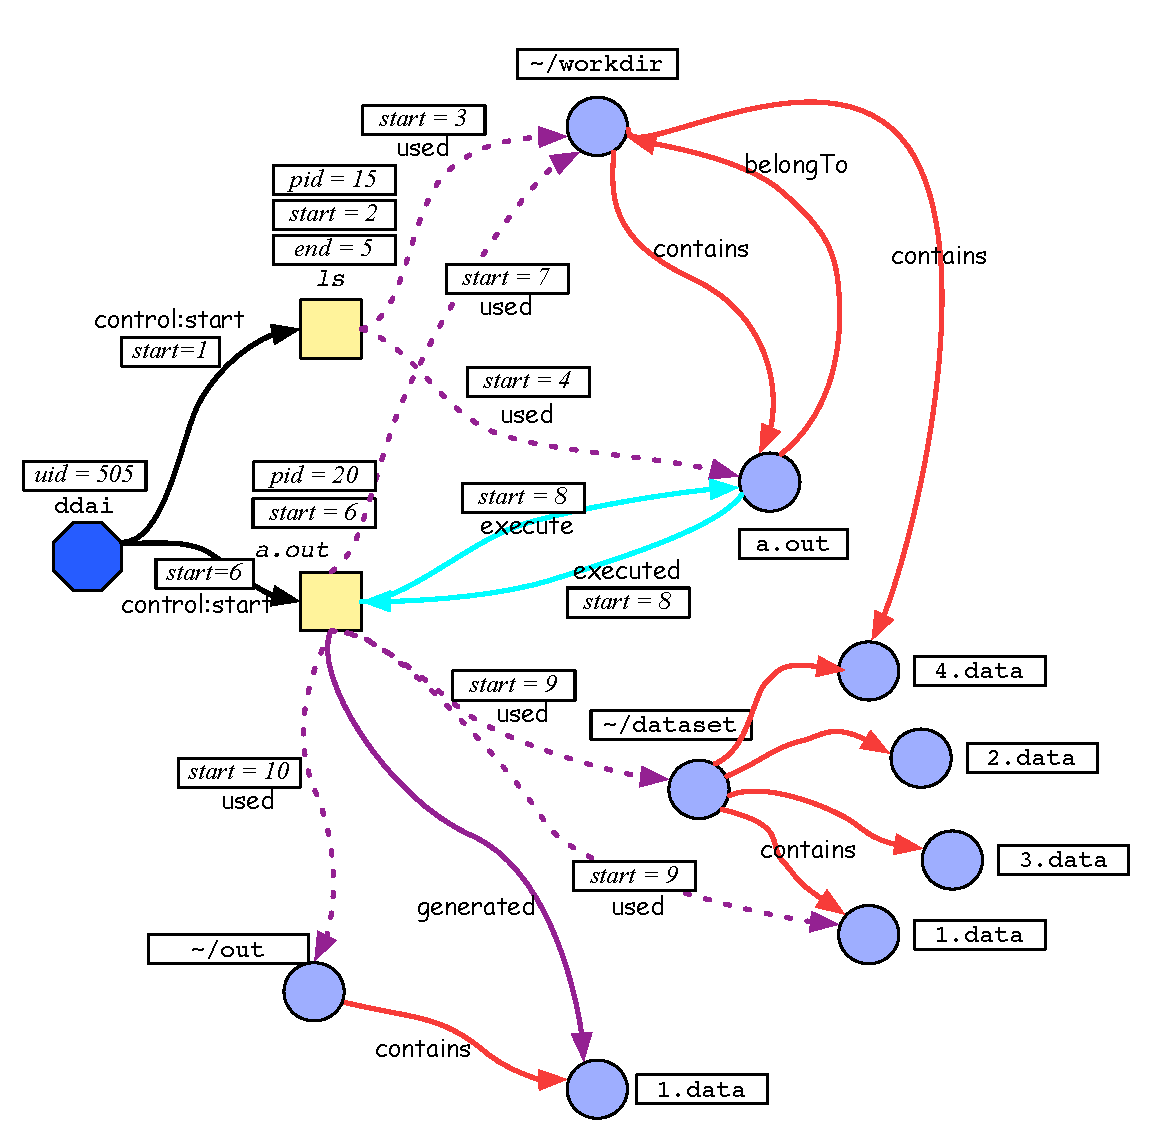
\includegraphics[width=3.2in]{images/exagraph.pdf}
   \caption{An example instance of metadata graph.}
   \label{exampleGraph}
 \end{center}
\end{figure}

Figure~\ref{exampleGraph} shows an example metadata graph, a user
named `ddai' with \textit{uid} $505$ executed two processes: \textit{ls} and
\textit{a.out} in order. First, he ran \textit{ls} in the `workdir' to
locate the executable file: `a.out'; after that, he started a process to
run this executable. The process will read data file under `dataset' with
name `1.data' and write data file under `out' with name `1.data' too. The
directory data object actually `contains' multiple other data objects.




\textit{gRMM} allows users to create their own relationships. The created relationships can be used to accelerate later query and
search. For example, given that a user `controls' a process, which will `use'
a data object, we can create a `visit' relationship between users and
data objects to record the visiting history of a user. This example is shown
in Fig.~\ref{nr}.

\begin{figure}[ht]
\begin{center}
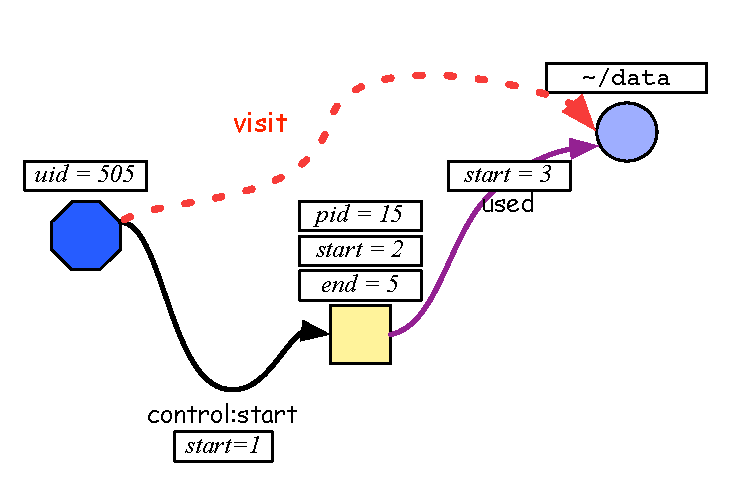
\includegraphics[width=3in]{images/newrelation.pdf}
\caption{An example of new relation named as \textit{visit}.}                                                                                  
\label{nr}
\end{center}
\end{figure}

There are two ways to create new relationship. The basic
way is to create an edge instance and connect it with
two existing vertice in the graph. This mechanism is mainly 
useful for relations that
cannot be inferred from existing relations. A simple example would be a
`recently created' relation between a data file and a user: whenever
a new file is created by a user, the application can add a specific
relation between them.

We also provide another way to create new relationships, called
\textit{combinations}. Users can submit a script that describes
how to combine existing relations to build a new one. For example,
generate a `visit' relation by combining `control' and `used'
relations as shown in Fig.~\ref{nr}. Submitting this script to 
\textit{gRMM} will trigger a distributed graph
task that results in the generation of new edges (relations).  The graph
will need to be submitted again to obtain updated results.
We will evaluate the practical implications of allowing users to submit
combination scripts to the system as well.  This feature may be restricted
to administrators for resource and security reasons.

In conclusion, the metadata graph model includes three basic predefined
entities and ten paired relations. Both the entities and relations contain unlimited user-defined properties which could be used as filter or search keywords.




\subsection{Graph Storage}

There are several choices to store metadata graphs. The first will be relation database, which was traditionally used to store provenance graph. However, storing graph in relation databases requires a complex scheme with multiple tables and foreign keys to refer each other. This introduces poor performance during traveling the graph as we need to do time-consuming `join' of different tables to build a complete path.

Comparing with relation databases, graph databases are more suitable. 

Another storage choice is Key-Value storage systems. Comparing with relation databases and graph databases, they do not have any scheme. Simply mapping the nodes and edges as different objects and store their properties as the value of these objects provides a plain strategy to store the metadata graph. 

@TODO: In this section, we can show the performance of different storage systems (RDBMS, GraphDB, KeyValue) in different scenarios (Insert, Locate, Traversal). 


\subsection{Graph Traversal and Query}
Graph traversal languages like Gremlin, Cypher are also supported in these graph databases for querying. 

The proposed metadata graph follows a property graph model, which is different from traditional graph that only contains simple weight value on each edge. The property graph needs to store both the graph structure, which indicates the connections between nodes, and the rich data associated with the graph including properties on both nodes and edges. So, traveling through the property graph is different from traditional graph: we should only travel through limited number of edges which satisfy certain conditions, for example the edges whose type is \textit{run} instead of going through all the out-edges. 

@TODO: Shall we discuss the detailed level of metadata? 

\subsection{Graph Processing}

@TODO: 




\begin{table}[h]
\caption{Graph database category.}
  \label{gdc}
\centering
\begin{tabular}{|c||c|c|c|c|}
\hline
\textit{\textbf{}}    & \textbf{\begin{tabular}[c]{@{}c@{}}Data \\ Storage\end{tabular}} & \textbf{\begin{tabular}[c]{@{}c@{}}Graph \\ Structure\end{tabular}} & \textbf{\begin{tabular}[c]{@{}c@{}}Query \\ Language\end{tabular}} & \textbf{Dist.} \\ \hline

\textit{AllegroGraph} & Disk                                                         & Simple                                                       & SPARQL       & Yes           \\ \hline
\textit{DEX}          & Disk                                                         & Property                                                     & API                   & Yes  \\ \hline
\textit{G-Store}      & Disk                                                             & Simple                                                        & SQL-based       & Yes         \\ \hline
\textit{HyperGraphDB} & Disk                                                         & HyperGraph                                                        & API           & Yes           \\ \hline
\textit{InfinitGraph} & Disk                                                             & Property                                                      & API         & Yes             \\ \hline
\textit{Neo4j}        & Disk                                                         & Property                                                      & Cypher                   & Partly \\ \hline
\textit{Titan}        & Disk                                                         & Property                                                      & Gremlin                  & Yes  \\ \hline
\end{tabular}
\end{table}


%We generally classify them into two categories: the graph databases and distributed graph processing frameworks. The graph databases focus on physically storing the graph and providing basic searching and querying functionalities to users. At the same time, the distributed graph processing frameworks aim at providing high level abstractions to write algorithms that perform traversals of the whole graph (e.g. communication detection, page rank evaluation).\\


\begin{table}[h]
\caption{Distributed graph processing framworks.}
  \label{dgpf}
\centering
\begin{tabular}{|c||c|c|}
\hline
\textit{\textbf{}}           & \textbf{\begin{tabular}[c]{@{}c@{}}Programming\\ Abstraction\end{tabular}} & \textbf{\begin{tabular}[c]{@{}c@{}}Storage \\ Format\end{tabular}} \\ \hline
\textit{Gigraph/Pregel}      & Vertex-centric                                                             & HDFS/HBase/Hive                                                    \\ \hline
\textit{GraphX}              & Spark-based                                                                & RDD                                                                \\ \hline
\textit{GraphLab} & Vertex-centric                                                             & HDFS/S3                                                            \\ \hline
\textit{X-Stream}            & Edge-centric                                                               & Customized Format                                                  \\ \hline
\textit{Gigraph+}            & GraphPartition                                                             & Customized                                                         \\ \hline
\end{tabular}
\end{table}


 \begin{figure}[!ht]
        \centering
        \subfloat[parablolic\label{fig:first}] {%
          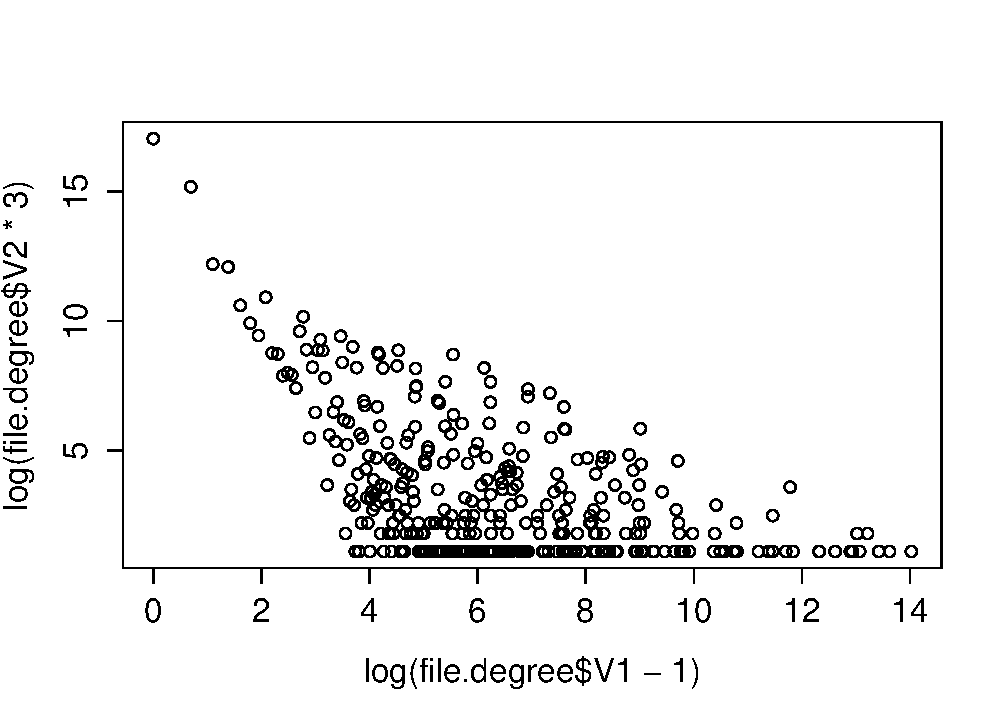
\includegraphics[scale=.35]{exps/rplot.pdf}
        }%
        \subfloat[npv1\label{fig:second}] {%
          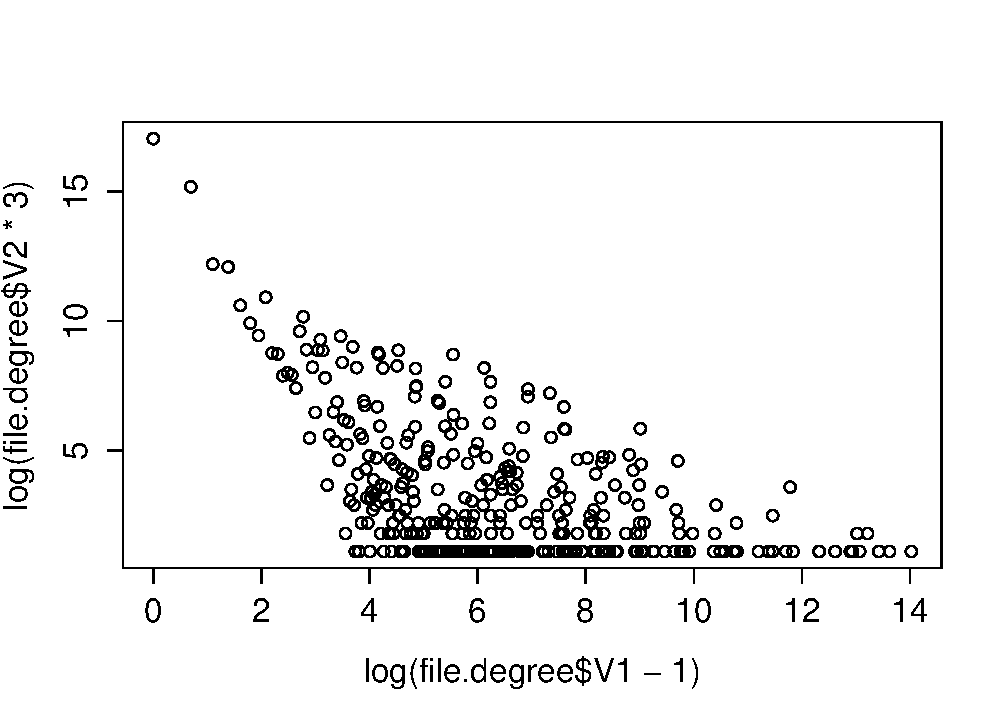
\includegraphics[scale=.35]{exps/rplot.pdf}
        } \\ %  ------- End of the first row ----------------------%
        \subfloat[npv2\label{fig:third}] {%
          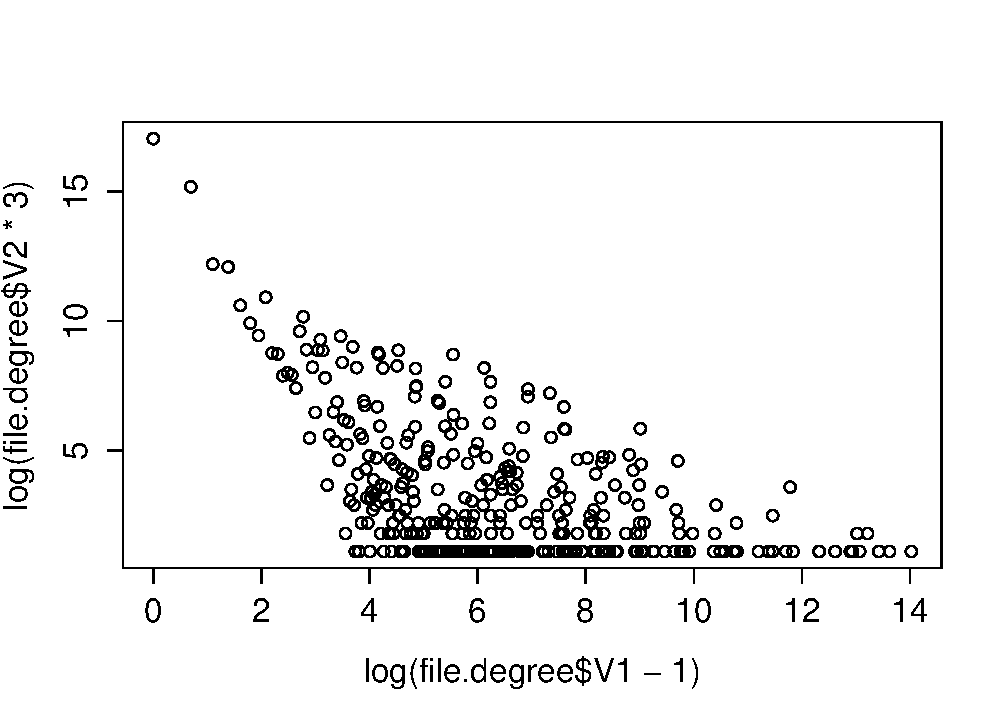
\includegraphics[scale=0.35]{exps/rplot.pdf}
        }%
        \subfloat[npv3\label{fig:fourth}] {%
          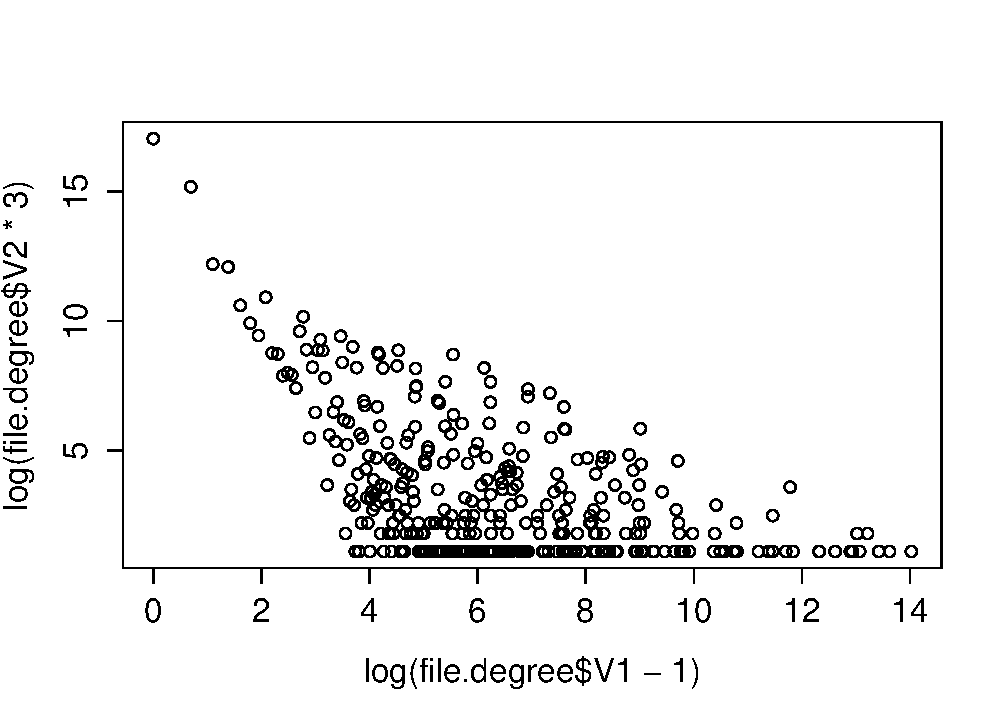
\includegraphics[scale=.35]{exps/rplot.pdf}
        }%
        \caption{The l-o-n-g caption for all the subfigures (FirstFigure through FourthFigure) goes here.}
        \label{fig:subfigures}
      \end{figure}